\chapter{有性生殖}\label{ch:g8:sexual-reproduction}

五月的蛙鸣，四月的樱花，秋日雄鹿的长吼，
以及朝向蜜蜂、满脸花盘的向日葵：
纵观整个\omterm{def:g6:exploring-our-environment:components}{生物}界，巨大的\omterm{prop:g3:balanced-diet:jobs}{能量}都投入到同一项事业上——
孕育下一代。前几年的课程分别讲过这些内容
（\cref{ch:g4:animal-reproduction}，
\cref{ch:g5:flower-to-fruit}）；本年将它们汇成一套理论，
并提出一个更尖锐的问题：为什么
偏偏要\emph{两}个亲本？

\begin{omfigure}
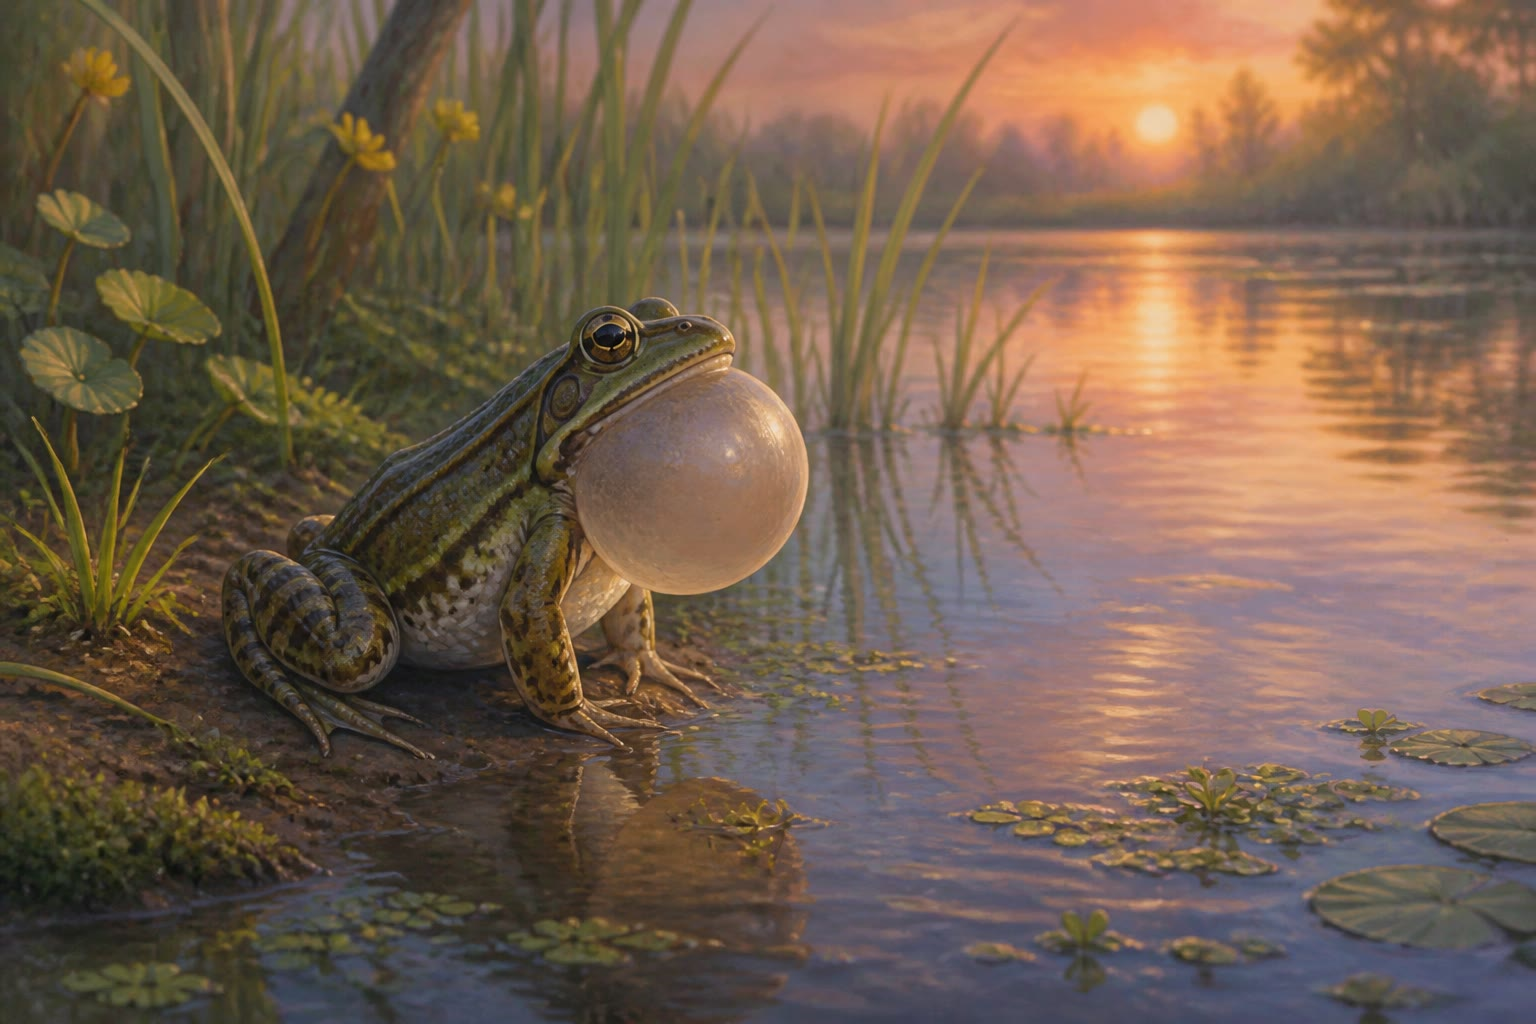
\includegraphics[width=0.6\linewidth]{images/book1/ai/g8-frog-chorus.jpg}

{\small 为同一项工程投入的巨大\omterm{prop:g3:balanced-diet:jobs}{能量}：\omterm{def:g4:animal-reproduction:sexual}{雄性}鼓起的声囊，
为\omterm{def:g8:sexual-reproduction:gametes}{配子}的相遇召集整片池塘。}
\end{omfigure}

\section{贯穿整个生物界的同一机制}

\begin{definition}[配子]\label{def:g8:sexual-reproduction:gametes}
由\cref{def:g4:animal-reproduction:sexual}所述的
生殖\omterm{def:g5:first-look-at-cells:cell}{细胞}统称为
\emph{配子}\index{配子}：雄配子（\omterm{def:g1:animals-around-us:animal}{动物}中为\omterm{def:g4:animal-reproduction:sexual}{精子}，
开花\omterm{def:g1:plants-around-us:plant}{植物}中为\omterm{def:g3:flowers-fruits-seeds:parts}{花粉}粒中的\omterm{def:g5:first-look-at-cells:cell}{细胞}）和
雌配子（即\omterm{def:g4:animal-reproduction:sexual}{卵细胞}，位于子房或\omterm{prop:g5:flower-to-fruit:roles}{胚珠}中）。
配子都是\omterm{def:g6:cell-unit-of-life:unicellular}{单细胞}
（见\cref{ch:g5:first-look-at-cells}），每一个都只是生命的一半起点：
独自时，配子会死去；结合后，两者便成就一个生命。
\end{definition}

\begin{proposition}[不变的核心]\label{prop:g8:sexual-reproduction:core}
凡\omterm{def:g4:animal-reproduction:sexual}{有性生殖}之处——\omterm{prop:g3:sorting-living-things:groups}{鱼类}或冷杉，
蜗牛或人类——其核心都是不变的：
\begin{enumerate}
  \item 两个亲本分别产生雄\omterm{def:g8:sexual-reproduction:gametes}{配子}和雌\omterm{def:g8:sexual-reproduction:gametes}{配子}；
  \item \emph{\omterm{def:g5:flower-to-fruit:steps}{受精}}：一个雄\omterm{def:g8:sexual-reproduction:gametes}{配子}与一个
        雌\omterm{def:g8:sexual-reproduction:gametes}{配子}结合，形成一个新\omterm{def:g5:first-look-at-cells:cell}{细胞}——
        \emph{\omterm{def:g5:flower-to-fruit:steps}{受精}后的\omterm{def:g4:animal-reproduction:sexual}{卵细胞}}，即
        \emph{受精卵}\index{受精卵}；
  \item \omterm{prop:g8:sexual-reproduction:core}{受精卵}反复分裂
        （见\cref{prop:g5:first-look-at-cells:growth}），
        发育成一个新个体，它携带着来自
        \emph{双方}亲本的某些特征
        （见\cref{rem:g4:animal-reproduction:mix}）。
\end{enumerate}
围绕这一核心，其余一切都只是变化：
\omterm{def:g8:sexual-reproduction:gametes}{配子}在何处相遇、数量多少、由谁照料幼体。
\end{proposition}
\admitted

\begin{example}[变化的分类]\label{ex:g8:sexual-reproduction:variations}
旧有的内容都可以整齐地归入这一核心之下。外部\omterm{def:g5:flower-to-fruit:steps}{受精}
与内部\omterm{def:g5:flower-to-fruit:steps}{受精}之别（见\cref{prop:g4:animal-reproduction:where}），
关乎相遇的地点。\omterm{def:g4:animal-reproduction:ovivivi}{卵生}与\omterm{def:g4:animal-reproduction:ovivivi}{胎生}之别
（见\cref{def:g4:animal-reproduction:ovivivi}），关乎\omterm{prop:g8:sexual-reproduction:core}{受精卵}的
栖身之所。鳕鱼的海量产卵与大象的单胎
（见\cref{prop:g4:animal-reproduction:strategies}），关乎数量的
账目。蜜蜂或风媒\omterm{def:g5:flower-to-fruit:steps}{传粉}（见\cref{def:g5:flower-to-fruit:steps}），
关乎雄\omterm{def:g8:sexual-reproduction:gametes}{配子}的运送服务。
同一机制，
不同情境构成的一份目录。
\end{example}

\begin{remark}[植物遵循同一核心]\label{rem:g8:sexual-reproduction:plants}
将\cref{ch:g5:flower-to-fruit}与
\cref{ch:g4:animal-reproduction}并置，两者完全吻合：\omterm{def:g3:flowers-fruits-seeds:parts}{雄蕊}与\omterm{def:g3:flowers-fruits-seeds:parts}{雌蕊}
产生\omterm{def:g8:sexual-reproduction:gametes}{配子}，\omterm{def:g3:flowers-fruits-seeds:parts}{花粉}管是体内\omterm{def:g5:flower-to-fruit:steps}{受精}的通道，
\omterm{def:g2:from-seed-to-plant:seed}{种子}内收藏着\omterm{def:g1:plants-around-us:plant}{植物}的胚，并备有储存的养料
（见\cref{def:g2:from-seed-to-plant:seed}）。只有\omterm{def:g4:plants-without-seeds:vegetative}{营养繁殖}
（见\cref{def:g4:plants-without-seeds:vegetative}）是例外——
仅一个亲本，无\omterm{def:g8:sexual-reproduction:gametes}{配子}，
产生完全相同的后代：这一对照
使下一节的问题
变得更加尖锐。
\end{remark}

\section{为什么需要两个亲本？}

\begin{proposition}[有性生殖促成重组]\label{prop:g8:sexual-reproduction:shuffle}
\omterm{ex:g4:plants-without-seeds:runner}{匍匐茎}繁殖的草莓复制株
（见\cref{rem:g4:plants-without-seeds:copy}）表明，
单亲的结果是完全相同。双亲则恰好相反。
每个\omterm{prop:g8:sexual-reproduction:core}{受精卵}都由双亲各出一个\omterm{def:g8:sexual-reproduction:gametes}{配子}结合而成——
后续章节将会说明，即便同一亲本的两个\omterm{def:g8:sexual-reproduction:gametes}{配子}，
遗传信息也不完全相同——
因此\omterm{def:g4:animal-reproduction:sexual}{有性生殖}使每个后代都获得一种
\emph{新的组合}。兄弟姐妹各不相同；
同一豆荚中的\omterm{prop:g2:from-seed-to-plant:cycle}{幼苗}没有两株完全一样；
每个\omterm{def:g5:biodiversity:species}{物种}内部的多样性（见\cref{rem:g5:biodiversity:scales}）
很大程度上便是这种重组的结果。
\end{proposition}
\admitted

\begin{example}[果园的两种赌注]\label{ex:g8:sexual-reproduction:bets}
（见\cref{rem:g4:plants-without-seeds:copy}）中的果园
两种方式都是有意为之。嫁接与\omterm{met:g4:plants-without-seeds:cutting}{扦插}：单亲，
完全复制优良的母树——同时也共享同一弱点，
一场枯萎病便可能一并毁掉全部。以果核播种：
双亲，每株\omterm{prop:g2:from-seed-to-plant:cycle}{幼苗}都是新的组合——多数平平，
有的较差，偶有一株优于双亲之一，
且彼此不同，枯萎病无法一网打尽。
复制保住的是现在，洗牌探索的是未来。
\end{example}

\begin{remark}[多样性是物种的储备]\label{rem:g8:sexual-reproduction:reserve}
这种重组为何超出果园的范畴而意义重大：
\cref{prop:g5:biodiversity:web}已指出，\omterm{def:g5:food-webs:web}{食物网}通过\omterm{def:g5:biodiversity:species}{物种}的多样性
吸收冲击；在同一\omterm{def:g5:biodiversity:species}{物种}之内，个体的多样性
发挥着同样的作用。当\omterm{def:g6:exploring-our-environment:components}{环境}发生变化——比如出现新的疾病，
或者冬季更加严酷——多样的\omterm{def:g5:biodiversity:species}{物种}更有可能
保有某个\omterm{def:g4:adapted-to-their-world:adaptation}{适应}新\omterm{def:g6:exploring-our-environment:conditions}{条件}的个体。这一点
对生命历史意味着什么，
\cref{ch:g9:how-species-change}将加以明确；
这里只需注意，\omterm{def:g4:animal-reproduction:sexual}{有性生殖}
正是维持这一储备的途径。
\end{remark}

\section{解读任何物种的生殖}

\begin{method}[生殖档案]\label{met:g8:sexual-reproduction:dossier}
对任何\omterm{def:g5:biodiversity:species}{物种}，整理以下各项：
\begin{enumerate}
  \item \omterm{def:g8:sexual-reproduction:gametes}{配子}：由谁产生何种\omterm{def:g8:sexual-reproduction:gametes}{配子}，在何处产生；
  \item 相遇：体外\omterm{def:g5:flower-to-fruit:steps}{受精}还是体内\omterm{def:g5:flower-to-fruit:steps}{受精}，以及
        运送方式（水、\omterm{prop:g4:animal-reproduction:where}{交配}、\omterm{def:g5:flower-to-fruit:steps}{传粉}者、
        风）；
  \item 居所：产卵还是携带幼体，配有何种
        储备；
  \item 数量与照料：该\omterm{def:g5:biodiversity:species}{物种}在策略谱系中的位置
        （见\cref{prop:g4:animal-reproduction:strategies}）；
  \item 季节：何时繁殖，由何种因素定时——
        下一章的问题。
\end{enumerate}
\end{method}

\begin{example}[两份档案并列]\label{ex:g8:sexual-reproduction:dossiers}
刺鱼（见\cref{exo:g4:animal-reproduction:10}）：
\omterm{def:g8:sexual-reproduction:gametes}{配子}排入水中，体外\omterm{def:g5:flower-to-fruit:steps}{受精}，卵产在
筑成的巢中，数十枚，由雄鱼守护，春季。
樱桃树：\omterm{def:g8:sexual-reproduction:gametes}{配子}在花中形成，体内\omterm{def:g5:flower-to-fruit:steps}{受精}，
\omterm{def:g3:flowers-fruits-seeds:parts}{花粉}管深入，\omterm{def:g5:human-reproduction:pregnancy}{胚胎}存于\omterm{def:g2:from-seed-to-plant:seed}{种子}中，
\omterm{prop:g3:flowers-fruits-seeds:transform}{果实}中，数以千计，获得养分后便交由
\omterm{prop:g3:sorting-living-things:groups}{鸟类}这一“运输服务”
（见\cref{exo:g6:how-plants-spread:12}），时间定在四月。
形式相同，适用于任何\omterm{def:g5:biodiversity:species}{物种}：档案即
理论的实际运用。
\end{example}

\section{练习}

\begin{exercise}[$\star$]\label{exo:g8:sexual-reproduction:1}
给出\omterm{def:g8:sexual-reproduction:gametes}{配子}与\omterm{prop:g8:sexual-reproduction:core}{受精卵}的定义，并分别写出\omterm{def:g1:animals-around-us:animal}{动物}和开花\omterm{def:g1:plants-around-us:plant}{植物}
的两种\omterm{def:g8:sexual-reproduction:gametes}{配子}名称。
\end{exercise}

\begin{exercise}[$\star$]\label{exo:g8:sexual-reproduction:2}
用三个步骤陈述不变的核心。
\end{exercise}

\begin{exercise}[$\star$]\label{exo:g8:sexual-reproduction:3}
请将下列各对归入核心：体外/体内\omterm{def:g5:flower-to-fruit:steps}{受精}，
\omterm{def:g4:animal-reproduction:ovivivi}{卵生}/\omterm{def:g4:animal-reproduction:ovivivi}{胎生}，数以百万计/仅一个——各对
变化的是什么？
\end{exercise}

\begin{exercise}[$\star$]\label{exo:g8:sexual-reproduction:4}
将\omterm{def:g1:plants-around-us:plant}{植物}部分与\omterm{def:g1:animals-around-us:animal}{动物}中的对应角色配对：\omterm{def:g3:flowers-fruits-seeds:parts}{雄蕊}、
\omterm{def:g3:flowers-fruits-seeds:parts}{雌蕊}、\omterm{def:g3:flowers-fruits-seeds:parts}{花粉}管、\omterm{def:g2:from-seed-to-plant:seed}{种子}。
\end{exercise}

\begin{exercise}[$\star$]\label{exo:g8:sexual-reproduction:5}
单亲生殖能产生哪些双亲生殖永远无法产生的结果——
反过来呢？
\end{exercise}

\begin{exercise}[$\star$]\label{exo:g8:sexual-reproduction:6}
兄弟姐妹为何彼此不同，
依据\cref{prop:g8:sexual-reproduction:shuffle}？
\end{exercise}

\begin{exercise}[$\star\star$]\label{exo:g8:sexual-reproduction:7}
解释果园的两种“押注”，
并说明各自在何时最为合适。
\end{exercise}

\begin{exercise}[$\star\star$]\label{exo:g8:sexual-reproduction:8}
请依照\cref{met:g8:sexual-reproduction:dossier}，
为青蛙整理生殖档案（全部材料见
\cref{ex:g4:animal-reproduction:song}和
\cref{ex:g2:animals-grow-up:frog}）。
\end{exercise}

\begin{exercise}[$\star\star$]\label{exo:g8:sexual-reproduction:9}
为蒲公英整理生殖档案——需注意一点：
许多蒲公英实际上未经\omterm{def:g5:flower-to-fruit:steps}{受精}便能结籽，
即借\omterm{def:g2:from-seed-to-plant:seed}{种子}实现克隆。哪些条目会
显得异常？这一反常对生殖档案
的整理有何启示？
\end{exercise}

\begin{exercise}[$\star\star$]\label{exo:g8:sexual-reproduction:10}
某葡萄园两百年来一直以\omterm{met:g4:plants-without-seeds:cutting}{扦插}繁殖一个著名的葡萄品种，
此时一种害虫入侵，恰好极爱该品种。
请将
\cref{ex:g8:sexual-reproduction:bets}改写为
该葡萄园的故事。
\end{exercise}

\begin{exercise}[$\star\star$]\label{exo:g8:sexual-reproduction:11}
“\omterm{def:g8:sexual-reproduction:gametes}{配子}是半个开端。”请对这一说法作两次论证：
一次依据核心的第 2 步，一次依据重组。
\end{exercise}

\begin{exercise}[$\star\star\star$]\label{exo:g8:sexual-reproduction:12}
为何能兼用两种方式的\omterm{def:g5:biodiversity:species}{物种}——草莓，
既有\omterm{ex:g4:plants-without-seeds:runner}{匍匐茎}\emph{又}有\omterm{def:g2:from-seed-to-plant:seed}{种子}——为何仍会两者都保留？请
为每种方式分配其功用，并利用
\cref{rem:g6:how-plants-spread:twospeeds}和
\cref{rem:g8:sexual-reproduction:reserve}。
\end{exercise}

\section{问题：育种计划}

\begin{problem}[{周末问题——一位植物育种者的一年，
依托理论展开}]\label{pb:g8:sexual-reproduction:1}
一位育种者想培育一种新苹果：口感脆爽如品种 A，
抗疫病如品种 B。她所用的工具恰好
正是本章所讲的内容。

\medskip\noindent\textbf{第一部分——杂交。}
\begin{enumerate}
  \item 她用刷子从 A 的\omterm{def:g3:flowers-fruits-seeds:parts}{雄蕊}上取\omterm{def:g3:flowers-fruits-seeds:parts}{花粉}，
        将\omterm{def:g3:flowers-fruits-seeds:parts}{花粉}涂到 B 的\omterm{def:g3:flowers-fruits-seeds:parts}{雌蕊}上，然后给花套袋，
        以防蜜蜂来访。请说明核心步骤中每一步的作用，
        以及套袋为何重要
        （\cref{met:g5:flower-to-fruit:diagnose}中用的
        正是同一把刷子）。
  \item 她授粉之后，B 的\omterm{prop:g3:flowers-fruits-seeds:transform}{果实}里会长出什么，
        而每粒\omterm{def:g2:from-seed-to-plant:seed}{种子}结合了哪两份遗传信息？
  \item 她播下三百粒\omterm{def:g2:from-seed-to-plant:seed}{种子}，为何预期会得到
        三百棵\emph{各不相同}的树，依据
        \cref{prop:g8:sexual-reproduction:shuffle}？
  \item 大多数\omterm{prop:g2:from-seed-to-plant:cycle}{幼苗}并不出众，少数还不如任一亲本，
        也许只有一株恰到好处。
        本章哪一个例子早已预测了
        这种分布？
\end{enumerate}

\medskip\noindent\textbf{第二部分——锁定优胜者。}
\begin{enumerate}[resume]
  \item 第八年：一棵树结出了口感脆爽、
        抗疫病的苹果。若她播下其\omterm{def:g2:from-seed-to-plant:seed}{种子}，
        这一珍贵组合会出现什么情况，
        为什么？
  \item 她改用嫁接的方法繁殖这棵优胜树，
——这属于哪种生殖方式，
        它能保证什么？
  \item 她未来整个果园，都将是这一棵树的
        无性系。请说出她所接受的风险，
        以及本章对此所用的术语。
  \item 提出\omterm{def:g3:sorting-living-things:criterion}{标准}的保险措施：她的果园还应保留什么，
        以及为何该策略会与
        品种储备相呼应（见
        \cref{rem:g8:sexual-reproduction:reserve}）？
\end{enumerate}

\medskip\noindent\textbf{第三部分——理论的
审查。}
\begin{enumerate}[resume]
  \item 她的方案先后用到了果园的两手策略。
        请说明各阶段用的是哪一手，
        以及各自为她带来了什么。
  \item 一位同事用同样的方式培育刺鱼，
——挑选亲本、培育重组后的
        幼体、留下最优者。请列出
        档案条目（\cref{met:g8:sexual-reproduction:dossier}）
        中\omterm{prop:g3:sorting-living-things:groups}{鱼类}做法与苹果做法不同的条目，
        以及核心步骤中不可能不同的
        步骤。
  \item 育种者说：“\omterm{def:g4:animal-reproduction:sexual}{有性生殖}提出方案，选择
        定夺——我只是在重组所给的
        结果中挑选。”请将她的这一口号
        与品种储备相联系，
        见\cref{rem:g8:sexual-reproduction:reserve}。
  \item 请用一句话作结：该方案
        需要\omterm{def:g4:animal-reproduction:sexual}{有性生殖}\emph{为了什么}，又
        为何需要\omterm{def:g4:plants-without-seeds:vegetative}{营养繁殖}？
\end{enumerate}
\end{problem}
